\chapter{Gerelateerd werk}
\label{hoofdstuk:related}
Het automatisch genereren van beschrijvingen voor ongeziene afbeeldingen is een complex proces. Het combineert namelijk zowel computervisie (CV) als natuurlijke taalverwerking (NLP). Vele modellen zijn al voorgesteld die telkens elementen uit beide onderzoeksvelden combineren. 

Dit hoofdstuk begint met een vergelijking van verschillende mogelijkheden om afbeeldingen en zinnen voor te stellen. De meest relevante onderzoeken uit CV en NLP komen aan bod. Daarna volgt een samenvatting van de verschillende mogelijkheden om deze technologie\"en te integreren in \'e\'en model. 

Doorheen de jaren is deze integratie op verschillende manieren aangepakt. Het probleem van automatische afbeeldingsbeschrijving werd eerst niet beschouwd als generatieprobleem maar als opvraag- of \emph{retrievalprobleem}. Hierbij zoekt een model naar de beste zin in een bestaande verzameling van zinnen op basis van de ingevoerde foto~\cite{Hodosh2013}. Nieuwere papers behandelen het probleem als een vertaalprobleem naar analogie met automatisch vertalen. Hierbij gebruikt men een codeer-decodeersysteem dat de afbeelding als brontaal beschouwt en het Engels als doeltaal. Dit hoofdstuk biedt een overzicht van deze recentste technieken.

\section{Representatie van afbeeldingen}
Alle recente modellen gebruiken technieken uit computervisie om nuttige kenmerken af te leiden uit afbeeldingen. Kenmerken bevatten onder andere gedetecteerde acties, sc\`enes en objecten met hun attributen en relaties~\cite{Bernardi}. Deze kenmerken vormen de basis voor een representatie van de afbeelding die als input dient voor het generatie- of opvraagmodel.

Eerst volgt een bespreking van technieken uit het verleden. Daarna beschrijft deze sectie Convolutionele Neurale Netwerken (CNN), die in de meer recente literatuur veelvuldig voorkomen.


\subsection{Oorspronkelijke CV modellen}
De literatuur gebruikt meerdere technieken uit computervisie om nuttige features of kenmerken af te leiden uit afbeeldingen. Kenmerken die in de vroegste papers over dit onderwerp voorkomen zijn bijvoorbeeld het type van de algemene sc\`ene, gedetecteerde objecten en attributen van deze objecten~\cite{Farhadi2010,Patterson2014,Yang2011}.

Bij sc\`eneclassificatie leert een model voor ongeziene afbeeldingen een bepaalde algemene sc\`ene (bijvoorbeeld restaurant, slaapkamer, keuken) af te leiden. Ook modellen die verschillende objecten detecteren hebben hun nut. Van zulke gevonden objecten kunnen classifiers ook nog nuttige attributen zoals kleur bepalen. Om zulke afleidingen te maken, gebruiken de papers bestaande classifiers en detectoren zoals bij Felzenswalb et al.~\cite{Felzenszwalb2008}, Im2Text~\cite{Ordonez2011} en GIST~\cite{Oliva2006}. Ee\'n of meerdere van deze features kan dan rechtstreeks de representatie vormen van een afbeelding. Daarnaast vormen deze features in een aantal werken~\cite{Farhadi2010,Li2011,Mitchell2012,Yang2011} enkel de input voor abstracte afbeeldingsrepresentaties in de vorm van tupels. Deze tupels bevatten dan objecten, acties tussen objecten, sc\`enetypes en/of ruimtelijke relaties. Figuur~\ref{fig:imgtriplets} geeft hiervan een voorbeeld.



Een andere manier om afbeeldingen voor te stellen is het gebruik van Visual Dependency Representations (VDR) zoals voorgesteld door Elliott et al.~\cite{Elliott2013}. Dit model werkt analoog aan een taalgebaseerde afhankelijkheidsgrammatica. Dit type grammatica stelt de syntactische structuur van een zin voor met woorden met daartussen binaire semantische of syntactische relaties~\cite{Jurafsky:2009:SLP:1214993}. Figuur~\ref{fig:dep_grammar} toont een voorbeeld van een zin ontleed met een afhankelijkheidsgrammatica. De gelabelde pijlen stellen de verschillende relaties tussen de woorden voor.

\begin{figure}[tb]
      \centering
      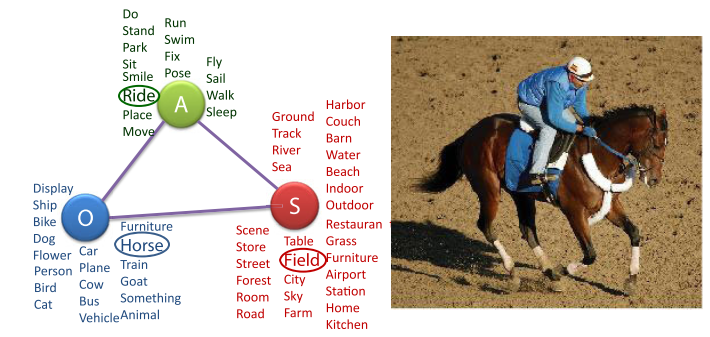
\includegraphics[width=\linewidth]{Images/imgtriples.PNG}
      \caption[Tripletrepresentatie van een afbeelding]{Tripletrepresentatie van een afbeelding waarbij elk triplet de vorm \texttt{<object(O),actie(A),sc\`ene(S)>} heeft. Verschillende detectoren leiden elk element in het triplet af uit de afbeelding.~\cite{Farhadi2010}}
      \label{fig:dep_grammar}
  \end{figure}  

VDR's gebruiken een afhankelijkheidsgraaf om de ruimtelijke relaties tussen regio's in een foto voor te stellen. Elke relatie tussen twee objecten krijgt dan een ruimtelijke positie als label. Mogelijke relaties zijn bijvoorbeeld \texttt{op}, \texttt{boven}, \texttt{onder}, \texttt{naast}, ... Het leren van VDR's kan op basis van geannoteerde trainingsdata, automatisch met objectherkenning~\cite{Elliott2015} of met nog andere informatie die in de abstracte sc\`ene zit~\cite{Gilberto2015}.  


\subsection{CV met neurale netwerken}
Naast deze meer traditionele manieren om informatie uit afbeeldingen af te leiden, bieden neurale netwerken een alternatieve oplossing. Voor een theoretische uitwerking van de gebruikte neurale netwerken, zie hoofdstuk~\ref{hst-theorie}.

Voor veel taken binnen computervisie blijkt dat convolutionele neurale netwerken (CNN) beter presteren dan bovenstaande methodes. Deze CNN's zijn deep learning neurale netwerken met soms meer dan 15 verborgen lagen. Ze hebben minder verbindingen en parameters dan overeenkomstige feedforward neurale netwerken terwijl ze niet veel slechter presteren~\cite{Krizhevsky2012a}. 
Voor verschillende CV-taken werken de huidige state-of-the-art oplossingen op basis van CNN's. Dit is onder andere het geval voor gezichtsherkenning~\cite{Zhou2015}, tekenherkenning~\cite{Ciresan2012} en objectherkenning~\cite{Szegedy2014}.

De gebruikte CNN's binnen het automatisch beschrijven van afbeeldingen zijn getraind op ImageNet~\cite{Russakovsky2014}. ImageNet is een dataset bestaande uit miljoenen afbeeldingen die gelabeld zijn binnen enkele duizenden categorie\"en. Het neuraal netwerk leert afbeeldingen correct te classificeren. Vaak gebruikte CNN modellen zijn AlexNet~\cite{Krizhevsky2012a} en het recentere VGGNet~\cite{Arge2015}.

Elke afbeelding dient als input voor het netwerk om zo tot een representatieve vector te komen. De meeste papers die afbeeldingen beschrijven gebruiken de gewichten van de laag voor de uiteindelijke classificatie als representatie van een afbeelding~\cite{Chen2014,Karpathy2015,Mao2014a,Google}. Aandachtsgebaseerde oplossingen~\cite{Jin2015,Xu2015} gebruiken ook de output van lagere convolutionele lagen als extra informatie.

Regionale CNN's vormen een variatie op CNN die een afbeelding opdeelt in verschillende interessante regio's. Hiermee is het mogelijk om voor elke regio een representatie te maken~\cite{Karpathy2015,Mitchell2015}. 

\section{Representatie van zinnen}
Het is niet eenvoudig om rechtstreeks met zinnen als een geheel te werken. Daarom zijn er verschillende alternatieven onderzocht om een zin voor te stellen.
De meeste modellen vertrekken van een vectorrepresentatie voor individuele woorden. In de literatuur zijn er verschillende manieren beschreven om woordrepresentaties samen te voegen tot een representatie van een zin.

\subsection{Voorstellen van woorden}
 Het voorstellen van woorden met een vector vergemakkelijkt de verdere verwerking en kan bovendien ook semantische informatie bevatten.

 Een eerste mogelijke voorstelling is een one-hot codering waarin een vector met als grootte het aantal woorden in het vocabularium elk woord voorstelt. Deze vector is volledig nul behalve op \'e\'en rij die overeenkomt met het woord. Het is mogelijk om deze representatie verder uit breiden door vermenigvuldiging met een gewichtsmatrix. Deze matrix transformeert de one-hotvectoren naar een andere vector. Training kan zorgen voor aanpassingen aan deze gewichtsmatrix om zo ook de semantische informatie van de woorden te leren. Op deze manier is elke rij in de matrix een vectorvoorstelling van een overeenkomstig woord. Deze gewichtsmatrix kan willekeurig worden ge\"initialiseerd of eerst trainen op bestaande corpora~\cite{Lebret2013,Mao2014a,Google}. Daarna kunnen de gekende woorden en zinnen uit de dataset de gewichten nog verfijnen.  

 Een andere mogelijkheid is om bestaande word embeddings te gebruiken zoals \texttt{word2vec}. Dat algoritme projecteert elk woord op een vooraf geleerde vector en heeft bovendien enkele mooie eigenschappen. Zo projecteert het semantisch gelijkaardige woorden op nabijgelegen posities in de vectorruimte~\cite{Mikolov2013}. Deze voorgedefin\"ieerde vectoren hebben als nadeel dat niet voor elk woord uit de beschrijvingen een vector representatie beschikbaar is. Het is wel mogelijk om zelf de vectorrepresentaties te leren op basis van de gebruikte dataset zoals beschreven in de paper.

 De meeste werken in de literatuur rapporteren dat one-hotcodering in combinatie met een te leren gewichtsmatrix gelijkaardige en snellere resultaten oplevert. Daarnaast hebben sommige semantisch gelijkaardige woorden zoals kleuren gelijkaardige vectoren bij gebruik van het \texttt{word2vec} algoritme, terwijl kleuren in een afbeelding toch uitgesproken verschillend zijn. Hierdoor zal een systeem dat \texttt{word2vec} woordvectoren gebruikt, waarschijnlijk slecht presteren in het herkennen van kleuren~\cite{Karpathy2015}.
 
\subsection{Voorstellen van zinnen}
 Verschillende mogelijkheden bestaan om de zinnen voor te stellen wanneer de woordvectoren gekend zijn. Een eerste mogelijkheid gebruikt een afhankelijkheidsparser en stelt de zinnen voor als een volledige afhankelijkheidsboom\cite{Socher2014}. Karpathy~\cite{Karpathy2014} gebruikt ook een afhankelijkheidsparser, maar haalt hier een verzameling van triplets uit. Dergelijke triplets bestaan uit twee woorden uit de zin en hun onderlinge relatie. Figuur~\ref{fig:deprelations} toont een voorbeeldzin met de bijhorende triplets. Het eerste element van de triplet is het type van de relatie.

 \begin{figure}[tb]
     \centering
     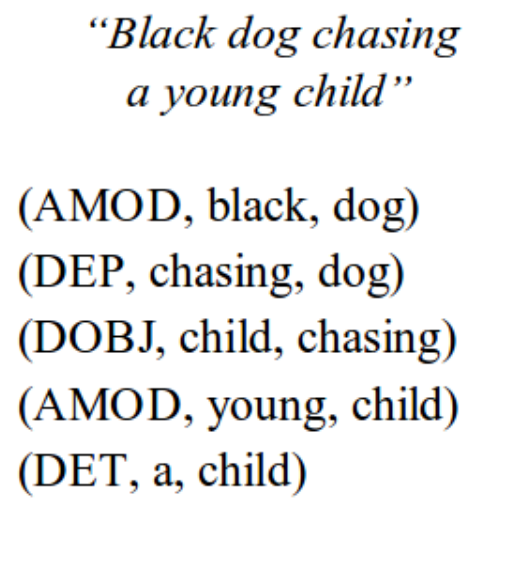
\includegraphics[width=0.35\textwidth]{Images/dep_relations}
     \caption[Zin met ontlede afhankelijkheidstriplets]{Zin met ontlede afhankelijkheidstriplets~\cite{Karpathy2014}. Het eerste element is de code van een type relatie tussen de twee volgende elementen.}
     \label{fig:deprelations}
 \end{figure}

 Een volgende optie telt de woordvectoren van een zin op~\cite{Lebret2013}  Hierdoor gaat informatie uit de woordvolgorde wel verloren. Le en Mikolov~\cite{Le2014a} bieden een oplossing voor het verloren gaan van woordvolgorde. Zij trainen een model om representaties te maken van stukken tekst met variabele lengte. Hun algoritme kan zowel zinnen als paragrafen en volledige teksten voorstellen.

 Een vaak gebruikt taalmodel in de meer recente NLP-literatuur is een Recurrent Neuraal Netwerk (RNN)~\cite{Mikolov2010}. Dit is een neuraal netwerk dat goed overweg kan met sequenti\"ele data zoals taal. Kiros et al.~\cite{Kiros2013} combineren de verborgen lagen van een RNN met extra informatie (zoals POS-tags) om tot een representatie van de zin te komen. De meer recente modellen stellen een zin voor als de sequentie van de woordvectoren in die zin. Zo kan het RNN de taal leren door elke zin woord per woord in het netwerk in te voeren.
 
\section{Van afbeeldingsrepresentaties naar beschrijvingen}
Er zijn verschillende methodes om vanuit de representaties van de afbeelding en bijbehorende referentiezinnen een model te trainen dat in staat is om ongeziene afbeeldingen om te zetten in correcte beschrijvingen. 
De meeste modellen trainen met als doel het verschil tussen de gegenereerde omschrijving en de correcte omschrijving uit de trainingsverzameling te minimaliseren.

\subsection{Dichtstbijzijnde afbeelding}
De eenvoudigste aanpak zoekt naar de meest gelijkaardige afbeelding in de trainingsverzameling en geeft \'e\'en van haar beschrijvingen terug als resultaat(Nearest Neighbour)~\cite{Devlin2015a}. Een gelijkaardigheidsmetriek zoals de cosinusgelijkenis tussen de afbeeldingsrepresentaties evalueert de gelijkaardigheid van twee representaties.

Een uitbreiding op deze aanpak zoekt naar de verzameling van de meest gelijkaardige afbeeldingen in de trainingsverzameling. Vervolgens cre\"eert een model een rangorde op basis van extra visuele of tekstuele informatie. De referentiezin van de hoogst scorende afbeelding is dan het resultaat~\cite{Devlin2015a,Hodosh2013,Oliva2006,Ordonez2011}. 
Deze modellen hebben als nadeel dat ze nooit resulteren in een zin die niet in de trainingsverzameling zit.

Een variatie hierop gebruikt een afbeeldingsvoorstelling met gedetecteerde objecten. Dit systeem zoekt naar de beschrijving van visueel gelijkaardige objecten in de vorm van zinsfragmenten (frases)~\cite{Gupta2012,Kuznetsova2012}. Met de verzamelde fragmenten zoekt het systeem dan de meest waarschijnlijke nieuwe zin op basis van het type van de fragmenten. Deze types bestaan uit naamwoordsgroep (NP), werkwoordsgroep (VP) en voorzetselgroep (PP). De samenstelling van een nieuwe zin gebeurt dus op basis van zinsdelen die objecten gelijkaardig aan die op de foto beschrijven. De auteurs defin\"ieren meerdere beperkingen op de gegeneerde zinnen om het aantal mogelijkheden te verkleinen.

Een andere variatie op Nearest Neighbour geeft de zinnen, samen met de dichtstbijzijnde afbeelding, als input aan een tweede model. Dit model vormt deze informatie dan om tot een nieuwe zin. Zo beschouwen Mason et al.~\cite{Mason2014} het genereren van beschrijvingen als een samenvattingsprobleem en gebruiken ze de beschrijvingen van gelijkaardige afbeeldingen als extra input. Analoog verkrijgen Jia et al.~\cite{Fernando2015} verbeteringen op bestaande modellen door het toevoegen van extra semantische informatie zoals beschrijvingen van gelijkaardige afbeeldingen op basis van Canonical Correlation Analysis (CCA).
 
\subsection{Multimodale modellen}
Enkele werken proberen een gemeenschappelijke ruimte tussen zinnen en afbeeldingen te leren zodat het mogelijk is om de representatie van zinnen zowel als afbeeldingen op dezelfde ruimte te projecteren. Dit laat toe om afbeeldingen en zinnen rechtstreeks te vergelijken met een afstandsmaat zoals bijvoorbeeld de cosinusgelijkenis. Dit is zeer nuttig voor onder andere het opvragen van afbeeldingen met een ongeziene query en zinnen met een ongeziene afbeelding. Het leren van multimodale modellen kan onder andere met Canonical Correlation Analysis (CCA)~\cite{Hodosh2013} en neurale netwerken~\cite{Mao2014,Karpathy2014,Kiros2013}. 

\subsection{Sjabloongebaseerd}
Een volgende aanpak baseert zich op sjablonen om zinnen te genereren. Op basis van de gebruikte afbeeldingsvoorstelling vult een algoritme een voorgedefinieerd sjabloon in~\cite{Yang2011}. Figuur~\ref{fig:sjabloon} geeft een voorbeeld van hoe deze paper een afbeeldingsvoorstelling met quadruplets omzet in een zin met een vaste structuur. Hiervoor is het dikwijls nodig om bijkomende complexe modellen te trainen~\cite{Elliott2013}. Het nadeel van deze methode is dat de gegenereerde zinnen wel syntactisch correct zijn, maar dikwijls onnatuurlijk aanvoelen voor mensen. Om deze methode te verbeteren kunnen gegenereerde of vooraf gekende zinsfragmenten helpen bij het hercombineren van fragmenten~\cite{Mitchell2012,Kuznetsova2012}. Daarnaast kan een algoritme een aantal gegenereerde zinnen sorteren op basis van bepaalde factoren en zo de beste zin eruit halen. Een voorbeeld van zulk systeem sorteert de zinnen op basis van hun waarschijnlijkheid in een vooraf geleerd taalmodel.

 \begin{figure}[tb]
 	\centering
 	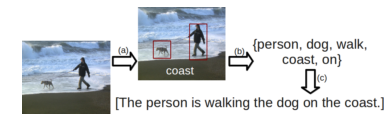
\includegraphics[width=\textwidth]{Images/sjabloon.PNG}
 	\caption[Overzicht van hoe een sjabloongebaseerd systeem werkt]{Overzicht van hoe een sjabloongebaseerd systeem werkt. (a) Detecteer objecten en sc\`enes uit inputafbeelding. (b) Schat bijbehorende optimale quadruplet van de vorm \texttt{\{objecten,werkwoorden,sc\`ene,voorzetsels\}}. (c) Vul met dit quadruplet een voorgedefini\"eerd sjabloon in.~\cite{Yang2011}}
 	\label{fig:sjabloon}
 \end{figure}

\subsection{Neurale netwerken}
De meest recente en best scorende modellen gebruiken neurale netwerken als taalmodel voor het genereren van beschrijvingen. Deze taalmodellen zijn in staat om compleet nieuwe, vlotte en natuurlijk aanvoelende zinnen te produceren. Vooral Recurrente Neurale Netwerken (RNN)~\cite{Mikolov2010} winnen in de literatuur aan populariteit als taalmodel. RNN's zijn in staat om sequenti\"ele data te genereren op basis van een zekere input. LSTM's (Long Short Term Memory)~\cite{SeppHochreiter1997} vormen een uitbreiding op de RNN's en onthouden informatie op lange termijn met behulp van een geheugencel. Deze masterproef maakt omwille van de goede prestaties in de literatuur ook gebruik van neurale netwerken om taal te genereren.

Beide modellen verwachten een sequentie van woordrepresentaties als input, maar kunnen ook uitgebreid worden met extra informatie als invoer. Zo gebruiken meerdere werken de afbeelding als eerste invoer. Een andere toevoeging cre\"eert een multimodale ruimte tussen afbeeldingen en zinnen~\cite{Kiros2014,Socher2014}. Xu et al.~\cite{Xu2015} voegen een ``aandachtsvector'' toe die aangeeft waar in de afbeelding het systeem moet focussen. Het is ook mogelijk om een combinatie van verschillende technieken te gebruiken, zoals het leren van een ``sc\`enevector'' in combinatie met een aandachtsgebaseerd systeem~\cite{Jin2015}. Jia et al. experimenteren met verschillende mogelijkheden om extra informatie toe te voegen, zoals CCA-projecties van afbeeldingen, of de afbeelding zelf~\cite{Fernando2015}.

Een eerste verzameling van modellen met neurale netwerken volgt het codeer-decodeerprincipe uit de automatische vertaling~\cite{Kiros2014}. De codeercomponent transformeert een afbeelding naar een nieuwe (multimodale) representatie. De decodeercomponent vertaalt vervolgens deze multimodale representatie naar een zin in natuurlijke taal. Door het multimodale karakter van deze modellen is het opvragen van afbeeldingen en zinnen ook mogelijk. Dit opvragen gebeurt door middel van projectie van een nieuwe afbeelding of zin in de multimodale ruimte. Een vergelijking van deze projectie met de zinnen of afbeeldingen uit de trainingsverzameling leidt tot een rangschikking van de trainingsvoorbeelden. Er bestaan zowel codeer-decodeer modellen met LSTM's~\cite{Kiros2014} als met RNN's~\cite{Karpathy2014,Mao2014a}.

Een tweede categorie gebruikt zowel de afbeeldingsrepresentatie als de sequentie van 
woordrepresentaties als input bij het trainen van het netwerk. Op basis van een trainingsafbeelding probeert het netwerk het eerste woord uit de zin te voorspellen. Deze voorspelling dient dan, al dan niet samen met de afbeelding, als input voor de voorspelling van het volgende woord. Terugpropagatie van de fout op de gegenereerde woorden doorheen het netwerk zorgt voor de juiste wijzigingen aan de gewichten. Op deze manier leert het netwerk om op basis van een ongeziene afbeelding de juiste sequentie van woorden te genereren. Ook hier bestaan er modellen met LSTM's~\cite{Donahue2015,Google,Xu2015} en RNN's~\cite{Karpathy2015,Mao2014a}.

Het trainen van deze netwerken gebeurt doorgaans met terugpropagatie doorheen het netwerk. Het is mogelijk om de fouten ook verder door te propageren naar de gewichtsvectoren van de woordrepresentaties of naar de gewichten van een CNN. Die methode optimaliseert op die manier alle gewichten op de dataset, maar kan computationeel kostelijk zijn.

Alle neurale netwerken gebruikt in deze thesis hebben een ``softmax'' als laatste laag. Deze laag zorgt ervoor dat het netwerk een kansverdeling genereert voor het volgende woord. Het meest waarschijnlijke woord heeft dan de hoogste kans.
Het selecteren van het woord voor de generatie kan gebeuren door het \emph{samplen} van deze verdeling of door het gebruik van een zoekalgoritme zoals beam search, om zo de meest waarschijnlijke beschrijving te benaderen. Samplen is het nemen van een willekeurig woord volgens de kansverdeling. Een specifiek stopwoord kenmerkt zowel het begin als het einde van de zin.

\subsection{Statistische taalmodellen}
Naast de neurale netwerken behoren ook de statistische taalmodellen tot de beter scorende modellen. Deze modellen proberen op basis van entropie een taal zo goed mogelijk te beschrijven. Entropie is een maat voor informatie en heeft verschillende doeleinden binnen het domein van NLP. 

Concreet stelt de entropie $H$ de hoeveelheid informatie voor die in een willekeurige variabele $X$ zit. $X$ is typisch de voorspelde variabele. Bij het afbeeldingsbeschrijvingsprobleem zijn dit typisch woorden of zinnen. Het domein van deze variabele is $\chi$. De entropie van $X$ is te berekenen met formule~\eqref{entropy}, waarbij $p(x)$ de kans voorstelt dat $X$ waarde $x$ heeft~\cite{Jurafsky:2009:SLP:1214993}. 

\begin{equation}
     H(X) = -\sum_{x \in \chi}p(x)\log_2p(x)
     \label{entropy}
 \end{equation} 

Entropie-gebaseerde modellen modelleren de kennis die zeker is en ze beschouwen onzekerheden als uniform. Als een woord vijf mogelijke vertalingen heeft, waar het systeem verder niets over weet, heeft elke vertaling een kans van $\frac{1}{5}$. Als het systeem uit observatie weet dat in 50 \% van de gevallen een van de eerste 2 vertalingen is, hebben deze twee vertalingen een waarschijnlijkheid van $\frac{1}{4}$. De andere drie vertalingen, waarover het systeem onzeker is, hebben een waarschijnlijkheid van $\frac{1}{6}$, wat neerkomt op een uniforme kansverdeling binnen de beperkingen die uit de observaties voortkomen. In andere modellen kunnen deze beperkingen voortkomen uit sjablonen en het al dan niet observeren van bepaalde woordsequenties, \ldots~\cite{Berger1996}

Zo leren Mitchell et al.~\cite{Mitchell2015} om een lijst met waarschijnlijke woorden uit de afbeeldingsrepresentatie te extraheren en combineren ze deze met een uitgebreid taalmodel. Dit taalmodel leert de verschillende kansen op basis van de beschrijvingen in de trainingsdata. Tijdens het leerproces probeert het algoritme de entropie te maximaliseren. Op deze manier leert het systeem steeds het meest waarschijnlijke distributiemodel gegeven de informatie die het al heeft gezien. In een volgende stap van hun systeem zoeken ze de zinnen die het meest waarschijnlijk zijn, gegeven de woorden die herkend zijn in de afbeelding. Vervolgens sorteren ze de gegeneerde zinnen op basis van een aantal additionele kenmerken. Dit model is net als de modellen met neurale netwerken in staat om nieuwe en vlotte zinnen te vormen. De prestatie is gelijkaardig aan die van de neurale netwerken.

Lebret~\cite{Lebret2015} toont bovendien aan dat een nog eenvoudiger taalmodel toch relatief goede resultaten kan bekomen. Dit model extraheert alle zinsfragmenten (frases) uit de trainingsdata en leert daarmee een eenvoudig 3-gram taalmodel. Voor ongeziene afbeeldingen bepaalt het model de best overeenkomende zinsfragmenten en probeert hiermee zinnen te maken. In tegenstelling tot alle voorgaande modellen gebeurt training van deze multimodale transformatie met \emph{negatieve sampling}. Hierbij leert het model een juiste referentiezin te onderscheiden in een lijst die ook willekeurig gekozen zinnen bevat. Ook hier gebeurt er aan het einde nog een hersortering van de gegenereerde zinnen op basis van de overeenstemming met de afbeelding.

\subsection{Aandachtsgebaseerde modellen}
State-of-the-art modellen uit het automatisch vertalen gebruiken mechanismes die aandachtsgebaseerd zijn. Concreet betekent dit dat het decodeeralgoritme zelf beslist welke stukken uit de zin meer aandacht vereisen.
In de setting van het beschrijven van afbeeldingen komt dit neer op een mechanisme dat aangeeft welke regio's in de afbeelding belangrijk zijn. In de decoder zorgt dit aandachtsmechanisme voor een extra contextvector als input voor een neuraal netwerk. 

Deze aandachtsvector kan zowel ``hard'' als ``zacht'' zijn. ``Harde'' aandacht is een stochastisch principe dat de aandachtslocatie beschouwt als een latente variabele. Tijdens elke stap samplet het algoritme \'e\'en locatie om de aandacht op te vestigen tijdens het genereren van het volgende woord. ``Zachte'' aandachtsmethodes werken deterministisch, waardoor er geen nood is om elke stap een sample-operatie uit te voeren. Een differentieerbare functie bepaalt de aandachtslocatie tijdens elke stap van het trainingsproces. Door de differentieerbaarheid is het netwerk dat de aandachtsvector berekent eenvoudig te trainen met behulp van terugpropagatie.

Aandachtsmodellen geven bovendien een mooie visuele voorstelling van waar het model bepaalde woorden ``ziet'' (figuur~\ref{fig:attention-example}). Binnen het automatisch beschrijven van afbeeldingen bereiken deze aandachtsgebaseerde modellen voorlopig de beste resultaten~\cite{Jin2015,Xu2015}.

\begin{figure}[tb]
	\centering
	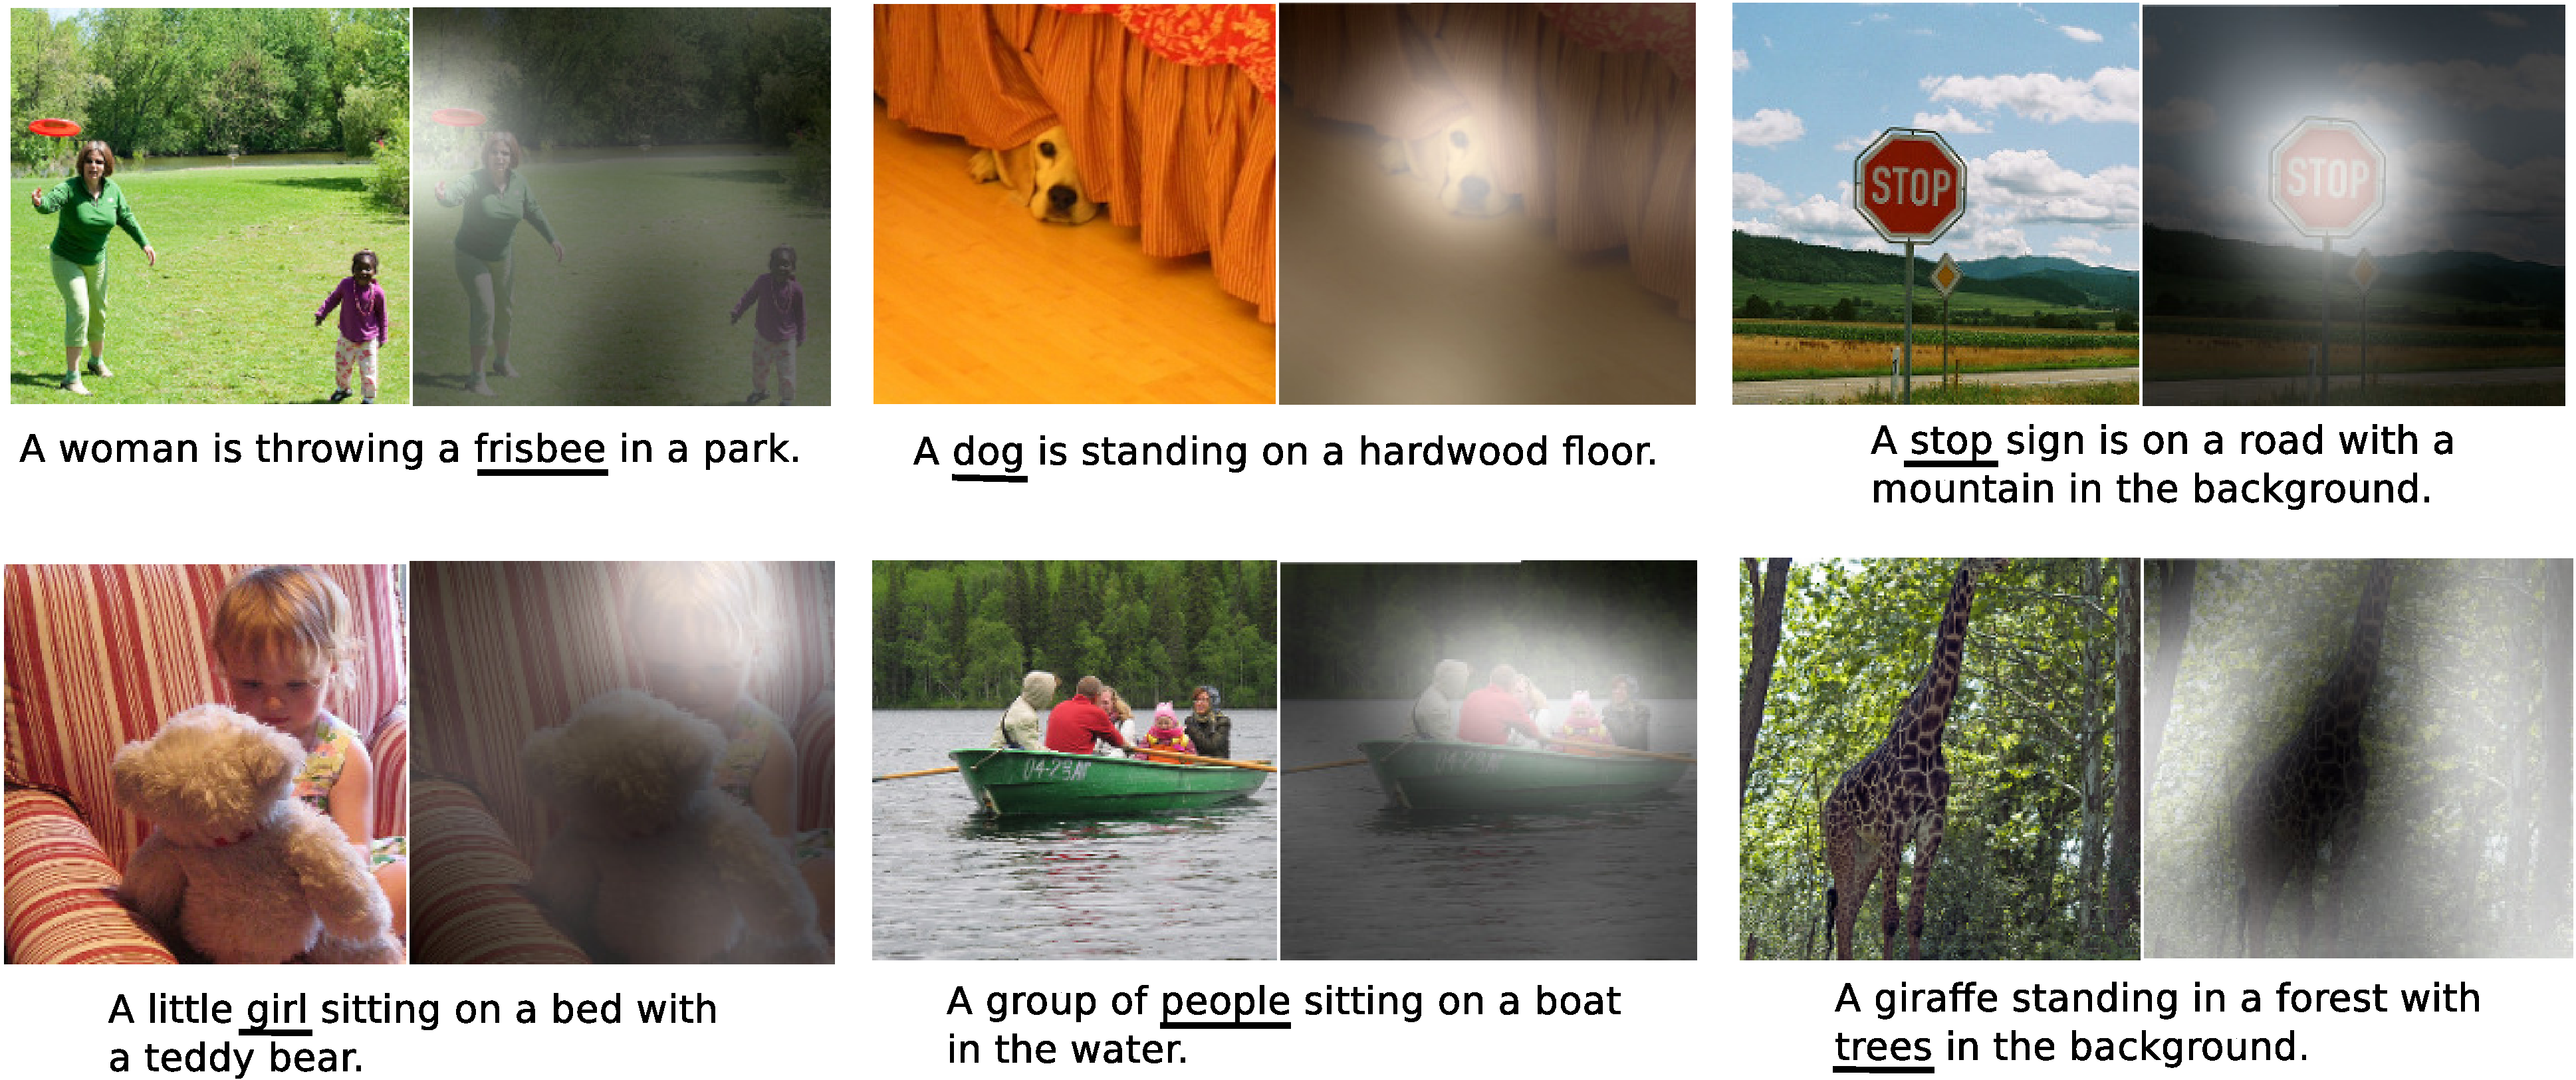
\includegraphics[width=\linewidth]{Images/good_Xu.pdf}
	\caption[Voorbeelden van aandacht op correcte regio.]{Voorbeelden van aandacht op correcte regio. (Wit in de afbeelding is de gefocuste regio, onderlijnde tekst is het overeenkomstige woord)~\cite{Xu2015}}
	\label{fig:attention-example}
\end{figure}


\section{Besluit}
Het probleem van deze masterproef bevat zowel elementen uit CV als NLP. Dit hoofdstuk bood een overzicht van hoe de literatuur componenten uit beide domeinen gebruikt om dit probleem op te lossen. Concreet vereist dit een voorstelling van zowel afbeeldingen als zinnen en een systeem dat hiermee afbeeldingsbeschrijvingen kan genereren. Zowel voor het beschrijven van afbeeldingen als het genereren van zinnen behalen neurale netwerken de beste resultaten. Om die reden gebruikt deze thesis dan ook respectievelijke CNN's en RNN's voor beide deelproblemen. Het volgende hoofdstuk gaat dieper in op de theoretische achtergrond van beide netwerken. Daarbovenop bespreekt dit hoofdstuk ook uitbreidingen op de netwerken en de toevoeging van extra semantische informatie om zo tot betere resultaten te komen.

%%% Local Variables: 
%%% mode: latex
%%% TeX-master: "masterproef"
%%% End: 